\chapter{Geometrische Modellierung}
\section{"`Rendering pipeline"'}
\begin{center}
 \rnode{geomodel}{Durchlaufen des geometrischen  \underline{\rnode{mod}{Modells}}\rput(3,1){\rnode{geo}{GEOMETRISCHE MODELIERUNG}}}\\[1em]
 \rnode{weltkoor}{Transformation von lokalen Modellkoordinaten in Weltkoordinaten}\\[1em]
 \ncline{->}{geomodel}{weltkoor}
 \rnode{kamerakoor}{Transformation in Kamerakoordinaten (NDC) (und Bildschirmkoordinaten)}\\[1em]
 \ncline{->}{weltkoor}{kamerakoor}
 \rnode{clipping}{Clipping: Abschneiden von teilen außerhalb des Sichtkegels}\\[1em]
 \ncline{->}{kamerakoor}{clipping}
 \rnode{beleucht}{Beleuchtung, Schattierung}\rput(3,0.5){\rnode{radiosity}{aufwändigeres Modell: RADIOSITY}}\\[1em]
 \ncline{->}{clipping}{beleucht}
 \rnode{z}{Bestimmen sichtbarer Flächen, Elimination verdeckter Flächen}\\[1em]
 \ncline{->}{beleucht}{z}
 \rnode{anzeige}{Anzeigen auf dem Bildschirm}\\[1em]
 \ncline{->}{z}{anzeige}
\end{center}
nur eine typische Reihenfolge!\\[1em]
Alle diese Operationen werden heute von Hardwareausgeführt\\[1em]
\ncline[linewidth=1.5pt]{->}{geo}{mod}
\ncline[linewidth=1.5pt]{->}{radiosity}{beleucht}
\ncangle[angleA=180,angleB=180]{<->}{beleucht}{z}\nbput{?}
\textbf{Alternative} für Beleuchtung, Schattierung und Bestimmung sichtbarer Flächen: Raytracing (Strahlverfolgung)

\section{Geometrische Modellierung}
\subsection{Wie kann man geometrische Formen darstellen?}
\begin{description}
 \item[Möglichkeit 1)] \emph{geometrische Grundformen} (Kugel, Zylinder, Polygone) werden zusammengesetzt\\[1em]
	Grundmodell: triangulierte Flächen.\\[1em]
	Mit triangulierten Flächen lässt sich im Prinzip alles genügend fein approximieren
	\begin{center}
	 16.1
	\end{center}
	(flache Polygone mit mehr als 3 Ecken sind in der Regel auch zugelassen)
	\begin{center}
	 16.2
	\end{center}
 \item[Möglichkeit 2)] \emph{Implizite Flächen} Fläche ist durch eine Gleichung gegeben
	\begin{center}
	 16.3
	\end{center}
	\[(x^2 + y^2)^2 + 3z^3xy - 28xz^2 = 0\]
 \item[Möglichkeit 3)] parametrische Fläche\\
	z. B. Kugel:
	\begin{align*}
	 x &= \cos \varphi \cos \vartheta\\
	 y &= \sin \varphi \cos \vartheta\\
	 z &= \sin \vartheta\\
	 0 \le \varphi \le 2 \pi \qquad & \qquad -\pi \le \vartheta \le \pi
	\end{align*}
\end{description}
\begin{center}
 \begin{tabular}{p{0.3\linewidth}|p{0.2\linewidth}|p{0.2\linewidth}|p{0.2\linewidth}}
  \textbf{Operation} & \textbf{Dreicksgitter} & \textbf{implizite Fläche} & \textbf{parametrische Fläche}\\
  \hline\hline
  Erzeugen eines Punktes auf der Fläche &
	sehr leicht & schwierig & sehr leicht \\\hline
  Durchlaufen aller Punkte der Fläche &
	sehr leicht & sehr schwierig & leicht \\\hline
  Schnitt der Fläche mit einem Sichtstrahl\newline
  (z. B. beim Raytracing)
	 & durchschnittlich\footnotemark[1] (Modell durchlaufen)
	 & leicht (Lösen eines Gleichungssystems in einer Variablen)
	 & sehr schwierig (Gleichungssystem mit 3 Variablen)\\\hline
  geometrische Manipulationen &
	sehr leicht & schwierig & durchschnittlich\\\hline
  Speicherverbrauch & ist abhängig von der Genauigkeit & kompakt & kompakt
 \end{tabular}
\end{center}
\footnotetext[1]{weder leicht noch schwer}
Umwandlung von impliziten oder paramtrischen Flächen in ein Dreicksgitter: "`Gittererzeugung"' ("`Meshing"')

\subsection{Darstellung polyedrischer Flächen bzw. Polygongittern}
\begin{enumerate}
 \item \textbf{primitiv:} Liste von Dreiecken, Vierecken, etc.
\begin{align*}
 D_1:\ &(x_1,y_1,z_1),(x_2,y_2,z_2),(x_3,y_3,z_3)\\
 D_2:\ &(x_4,y_4,z_4),(x_5,y_5,z_5),(x_6,y_6,z_6)\\
 \vdots\ 
\end{align*}
\begin{center}
 12.4 + 5
\end{center}
\paragraph*{Problem:} in einem typischen Dreiecksgitter kommen die gleichen Punkte mehrfach vor. Es ist
	Verschwendung, die gleichen Daten mehrfach zu speichern bzw. zu übertragen.
\item	Trennung der Koordinaten von der kombinatorischen Struktur:
	\begin{align*}
	 P_1:\ &(x_1,y_1,z_1) & D_1:\ &1,2,4\\
	 P_2:\ &(x_2,y_2,z_2) & D_2:\ &2,3,4\\
	 \vdots\ &		& \vdots\ 
	\end{align*}
	Flächen sind typischerweise \emph{orientiert}: Dreieck $P_1,P_2,P_3$ und Dreieck $P_1,P_3,P_2$ sind Vorder-
	und Rückseite des gleichen Dreiecks im Raum, un sie können unterschiedliche Materialeigenschaften haben.
	\begin{center}
	 16.6
	\end{center}
	Um noch mehr zu sparen, werden Dreiecke zu alternierenden Dreiecksstreifen bzw. Dreiecksfächern zusammengefasst.
	(und Vierecke zu Vierecksstreifen)
	\begin{center}
	 16.7
	\end{center}
	Für $n$ Dreicke benötigt man nur $n+2$ Punkte. Für isolierte Dreicke werden 3$n$ Punkte benötigt.
\end{enumerate}
\subsubsection{Datenstruktur zum Speichern der kombinatorischen Struktur einer polyedrischen Fläche}
\begin{itemize}
 \item Doubly-connected edge list (\emph{DECL}, doppelt-verkettete Kantenliste)
 \item Quad-edge data structure
 \item "`winged-edge"' data structure
\end{itemize}
Jede Kante wird durch zwei \emph{Halbkanten} repräsentiert, eine in jede Richtung
\begin{center}
 16.8
\end{center}
Jede Halbkante hat 3 Zeiger:
\begin{itemize}
 \item $l(e), r(e),...$ linke und rechte Nachbarkante mit demselben Startknoten
 \item $u(e)...$ Umkehrkante
\end{itemize}
\begin{center}
 16.9
\end{center}
\[
 \begin{array}{c||c|c|c}
  e & r(e) & l(e) & u(e)\\
  \hline\hline
  1 & 2 & 3 & 4\\
  2 &\emptyset & 1 & 5\\
  3 & 1 & \emptyset & 6\\
  4 & 7 & 8 & 1\\
  \vdots & \vdots & \vdots & \vdots
 \end{array}
\]
\begin{itemize}
\item Jede Kante liegt an bis zu 23 Flächen an, eine links und eine rechts.
\item Durchlaufen aller Kanten, die von einem Knoten ausgehen
\item Wir benötigen eine erste Kante $e_1$
	\begin{align*}
	 e_2 &= r(e_1)\\
	 e_3 &= r(e_2)\\
	&\ \vdots
	\end{align*}
	bis $e_i = e_1$ oder $e_i = \emptyset$
\end{itemize}
Durchlaufen aller Kanten einer Fläche, die rechts von $e_1$ liegt.
\begin{align*}
 e_2 &= l(u(e_1)) \\
 e_3 &= l(u(e_2)) \\
     &\ \vdots
\end{align*}
bis $e_i = e_1$
\begin{align*}
 l(r(e)) &= e & \text{falls } r(e) &\neq 0\\
 r(l(e)) &= e & \text{falls } l(e) &\neq 0\\
 u(u(e)) &= e
\end{align*}
\begin{center}
 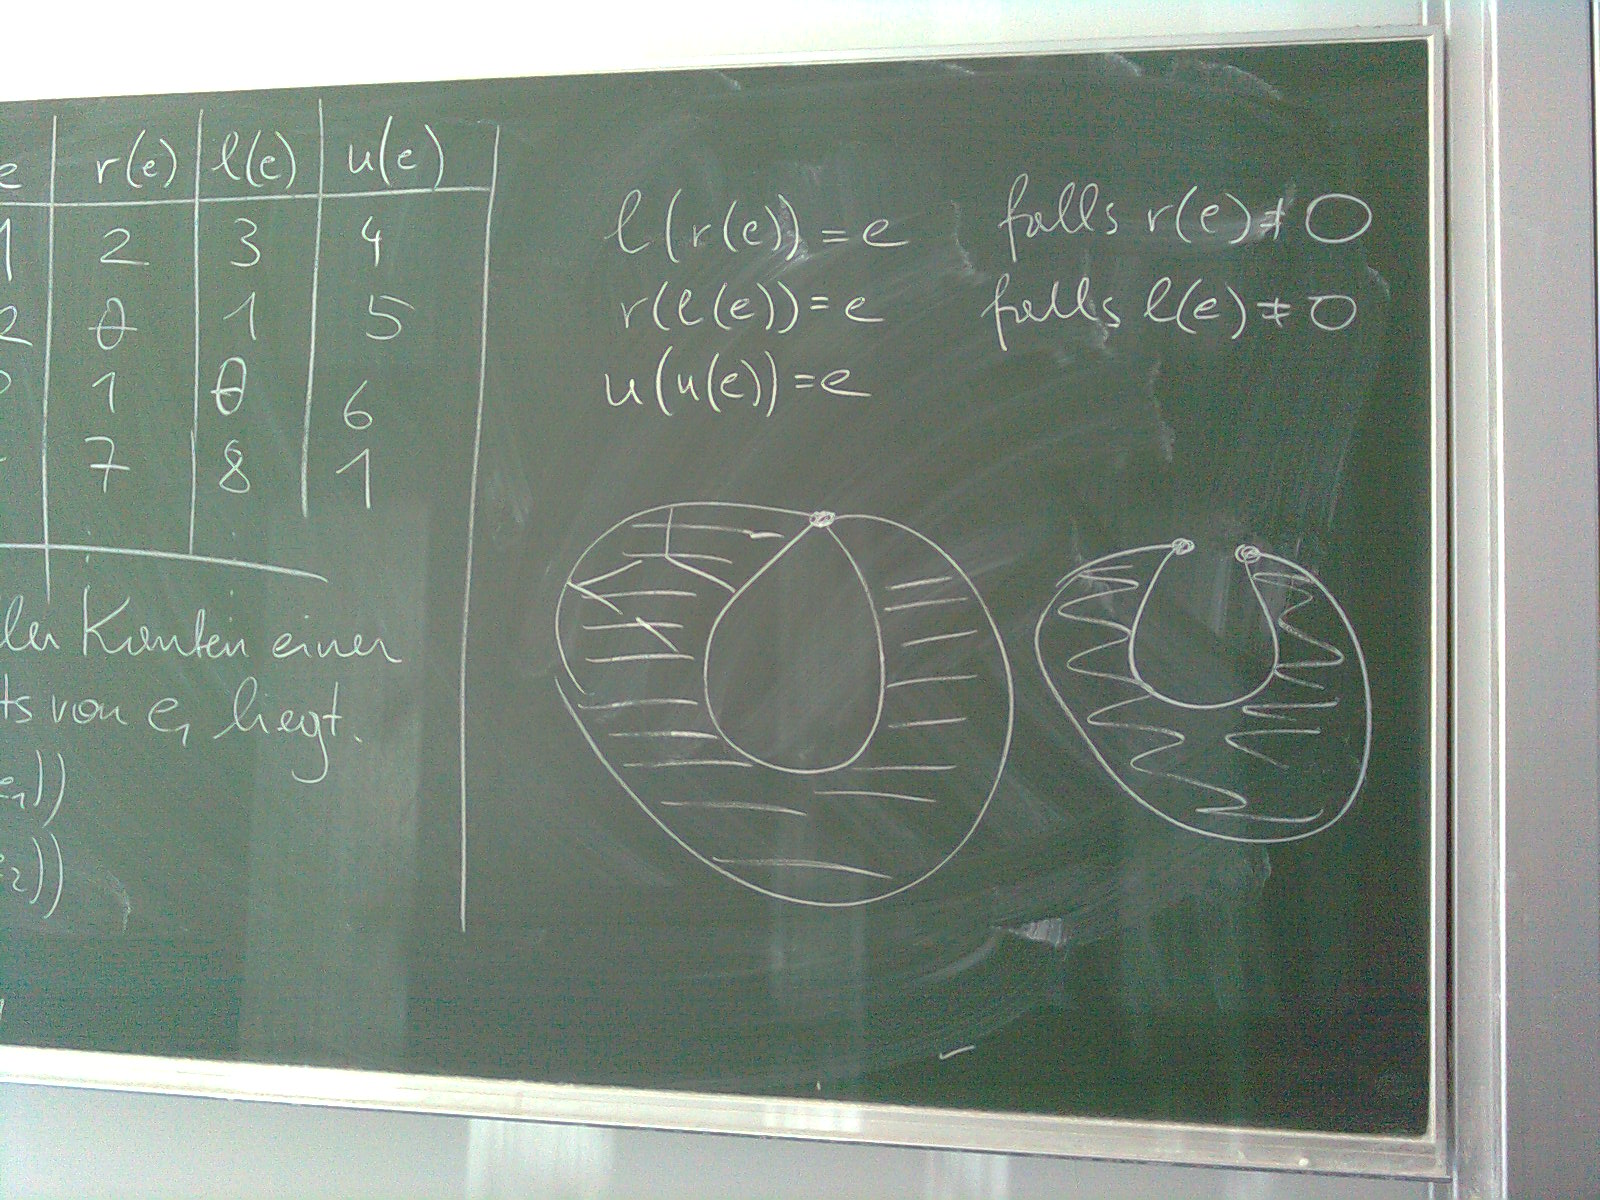
\includegraphics[width=\linewidth]{Foto-20100604-01.eps}
\end{center}

